%%!TEX root=../main.tex

\section{Workflow}

\subsection{Image Preprocessing}
The raw image from the dataset contains a lot of information where 
they are not necessary info the character recognition stage needs.
Therefore, we have to isolate the pixels related to the license 
plate so that we don't pass too many noise to the character recognition
part.

The first step is to figure out the location of licence plate in 
the whole picture. Related details regarding edge detection has been
mentioned back in background section. After we can draw a bounding box 
on the location of the license plate, we apply a binarization on the 
bounding area. An visualization of the mentioned workflow can be seen in 
Figure \ref{fig:preprocessing_image}. 

After obtaining the binary picture of licence plate, we then segment 
it into multiple pictures of individual characters. We can then 
obtain 7 independent character images which contains the abbreviation of 
province, letters and numbers.

As for the structure of a Chinese civil licence plate, it mainly consists 
of one Chinese character which is the abbreviation of province, follows by a 
letter from A to Z, which refers to the code-name of the area. 
For example, A normally refers to the capital of the province and 
finally following by 5 characters which are combinations of digits 
and letters(except O and I).

Applying the above-mentioned workflow to the whole raw data set allow us 
to generate a large number of single character images. Classification and
labelling are done through a script using the meta-info contained in the 
images' filename, including the province, letters and numbers. This step
allows us to prepare the dataset and CSV files for training the CNN used 
for classification.

According to the regular structure of a Chinese civil licence plate, 
We divide these character images into three categories:
\begin{enumerate}
    \item Province
    \item Area
    \item Letter
\end{enumerate}

The pre-processed dataset contains the following:
\begin{enumerate}
    \item 13175 samples and 34 classes in letter category
    \item 6713 samples and 26 classes in area category
    \item 2779 samples and 31 classes in province category
\end{enumerate}
In each of the categories, the samples are separated into a 
validation set, a training set and a testing set.
The training and testing sets are for training the CNN models while
the validation set is for evaluating the final accuracy of the models
being trained. 

\begin{figure}[t]
\centering
\subfloat[][Location of the licence plate]{
    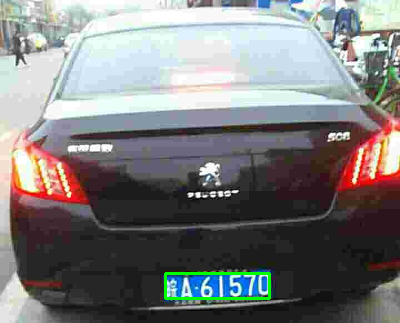
\includegraphics[width=1.5in]{\FIGDIR/03_preprocess_01.png}
    % \label{fig:subfig1}
}
\qquad
\subfloat[][Image after cropping]{
    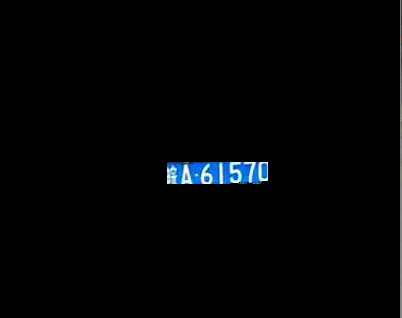
\includegraphics[width=1.5in]{\FIGDIR/03_preprocess_02.png}
    % \label{fig:subfig2}
}
\qquad
\subfloat[][Image after binarization]{
    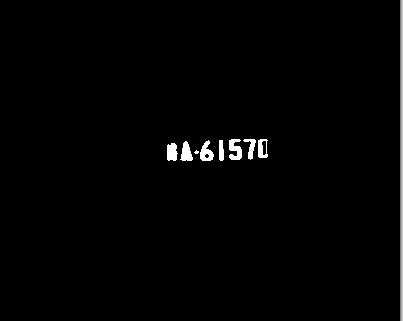
\includegraphics[width=1.5in]{\FIGDIR/03_preprocess_03.png}
    % \label{fig:subfig3}
}
\qquad
\caption{Example flow of the license plate image pre-processing}
\label{fig:preprocessing_image}
\end{figure}

\subsection{Sparse Preprocessing}
The training images will used to learn a convolution dictionary
and the sparse coding will be generated using the learned 
dictionary. Details on the algorithm being used was mentioned 
in the last section.

\subsection{Classifier}
We choose CNN to classify the character images.
Conventional Neural Network is a class of deep neural networks, 
which has a good performance on analyzing visual imagery.
As mentioned before, we have three categories of images, so we intend 
to train three independent models on these data. For letter and area, 
the character are letters and digits which their strokes are not complex.
Therefore, the architecture of the network dealing with these two categories
are similar which will be containing only two convolution layers and two dense layers.

For the province category, the Chinese characters considerably more complex
and harder to classify than letters and numeric digits, 
so we follow a more complex architectures which is similar to 
VGG16 \cite{simonyan2014very}. 

Figure \ref{fig:CNN_architecture} shows a simplified version of the
architecture of networks we are planning to use.

\begin{figure}[t]
\centering
\subfloat[][Architecture of the network of letter and area]{
    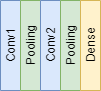
\includegraphics[width=1.0in]{\FIGDIR/03_CNN_arch.png}
    % \label{fig:subfig1}
}
\qquad
\subfloat[][architecture of network of province]{
    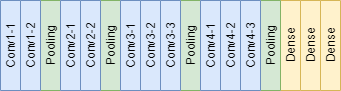
\includegraphics[width=2.25in]{\FIGDIR/03_CNN_arch_province.png}
    % \label{fig:subfig2}
}
\qquad
\caption{Example flow of the license plate image pre-processing}
\label{fig:CNN_architecture}
\end{figure}

\paragraph{CNN-Sparse-based method}
Considering sparse coding as pre-processing procedure to the images, 
we still want to compare the impact of different inputs on the performance of CNN model.
We intend to use the similar network architecture to training on the sparse representing dataset.

\paragraph{SVM-Sparse-based method}
In order to check if other machine classification methods could perform well 
on classifying licence plate, SVM is introduced. The main principle of SVM is that 
for linear data, it will find a hyper-plane to separate different classes and 
maximize the geometric spacing of each. 
It could also efficiently perform a non-linear classification by using kernel which 
will implicitly turn inputs into high-dimensional feature spaces.